\chapter{Relevant Teori for Design og Implementation}

I det følgende kapitel beskrives den teori, der ligger til grund for tilblivelsen af løsningsdesignet og implementationen af dette. Beskrivelsen af teorierne går ikke i dybden med emnerne, men har til formålet at give læseren en basal introduktion til teorierne, der er anvendt under udviklingen af løsningen. Grundet dette uddybningsniveau, er kun det mest relevante teori, for forståelsen af løsningen, medtaget, og der afholdes fra diskussion af disse teorier.

\section{Use Cases}

Udviklingen af løsningen er sket på baggrund af de forudgående analyser, samt diskussioner og overvejelser omkring mulige vinkler hvorfra problemet kan gribes an. Som en del af processen blev der udarbejdet use cases.

Det gøres for at udpensle sandsynlige arbejdsmønstre for den tiltænkte løsning, og for at normalisere ideer om interaktion med systemet.

Der er mange forskellige tilgange til use cases, men de tager udgangspunkt i det samme princip. I denne rapport er use cases lavet efter kapitel 17 i \enquote{Agile Principles, Patterns, and Practices in C\#} \cite{martin2006agile}. Denne bog er valgt fordi den har en simpel tilgang til use cases. Her følger en beskrivelse af use cases som præsenteret i \cite{martin2006agile}.

En use case er i simpleste forstand en følge af trin, der bliver udført mellem en person, kaldet aktøren, og et system. Traditionelt er en use case skrevet meget udførlig, men \cite{martin2006agile} mener at use cases handler om, at skrive det primære forløb af interaktionen. Ved at gøre det simpelt, sikres det, at der ikke bliver brugt tid på at diskutere punkter, der ikke er essentielle.

Trin i use cases tager udgangspunkt i et problemfrit forløb. Dertil kan skrives et alternativt forløb til sandsynlige afvigelser fra den problemfrie brug.

\subsection*{Use Case Diagram}

For at visualisere et systems use case, opsættes et use case diagram. Dette diagram visualiserer de aktuelle aktøre samt systemet og dets funktioner. I diagrammet er systemet repræsenteret som en aflang rektangel, og use cases repræsenteres af de ovale cirkler. Alt inden for rektanglet er systemet som er udviklet. Uden for systemet ses aktørerne samt hvilke use cases de kan interagere med, som er repræsenteret af linjerne. En af fordelene ved at lave dette diagram, er at der skabes et overblik, samt en bedre forståelse af hvilke aktørere der interagere med hvilke use cases. Diagrammet kaldes ofte for et \enquote{System Boundary Diagram} fordi det effektivt visualisere et systems grænser. På \cref{fig:usecase} ses et use case diagram for LOBOP.

\begin{figure}
  \centering
    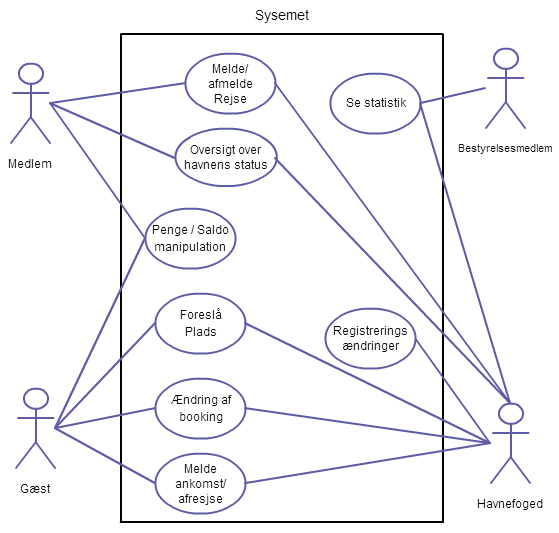
\includegraphics[width=\textwidth]{use_case_diagram.png}
  \caption{LOBOP System boundary diagram}
  \label{fig:usecase}
\end{figure}
\section{Internet of Things} % (fold)
\label{sec:internet_of_things}
Som en del af løsningen skal der indgå en sensorer, der kan detektere både i havnen. For at finde ud af mere, om hvad der er muligt, er konceptet \enquote{Internet of Things}, herefter IoT, blevet undersøgt. IoT er et paradigme, hvor alle fysiske genstande skal være unikt identificerbare, således at computere nemmere kan administrere disse genstande. Derudover handler IoT om at forbinde disse genstande i et netværk \cite{kopetz2011real}. En mere beskrivende definition af IoT er derfor \enquote{a world-wide network of interconnected objects uniquely addressable, based on standard communication protocols} \cite{iot_survey_2010}.

\subsection{Konceptet}
\label{sub:iot_koncept}
IoT er ofte beskrevet ud fra forskellige visioner for paradigmet. I \cite{iot_survey_2010}  beskrives tre visioner; \enquote{Things oriented}, \enquote{Internet oriented} og \enquote{Semantic oriented}. Disse visioner er opstået ud fra de forskellige interessenter i IoT. Disse interessenter angriber IoT fra forskellige vinkler og er derfor kommet fra til forskellige definitioner af IoT. Se \cref{fig:iot_visions}.

Den første definition af IoT, \enquote{Things oriented}, stammer fra Auto-ID labs, et verdensomspændende netværk af forskere indenfor Radio Frequency IDentification (RFID) og anden sensor teknologi. Målet med IoT er i denne definition at forbedre synligheden og muligheden for at spore genstande. For at opnå dette er Electronic Product Code (EPC) standarden blevet udviklet. Denne standard har til formål at sprede brugen af RFID samt andre teknologier \cite{iot_survey_2010}.

Den anden vision for IoT, \enquote{Internet oriented}, bygger videre på den første definition. Denne vision består i, at alle objekter selv kan forbinde sig til hinanden og computere. Konsortiummet CASAGRAS har fokus på at skabe \enquote{a world where things can automatically communicate to computers and each other, providing services to the benefit of the human kind} \cite{iot_survey_2010}.

Den sidste vision der beskrives her, \enquote{Semantic oriented}, omhandler hvordan de data, der genereres i \enquote{Things oriented} delen af IoT, organiseres. Visionen behandler strukturering af store mængder data, med hensigten at der opnås en forbedret overskuelighed og menneskelig forståelse, af disse ellers ofte overvældende mængder data \cite{iot_semantics_2012}.


\begin{figure}
  \centering
  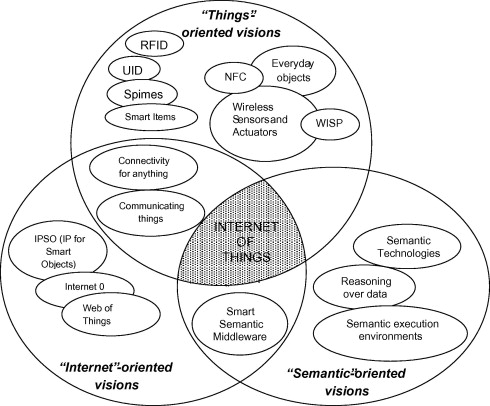
\includegraphics[width=\textwidth]{iot_visions}
  \caption{Internet of Things paradigmet ud fra tre visioner. Fra \cite{iot_survey_2010}.}
  \label{fig:iot_visions}
\end{figure}

\subsection{RFID}
RFID står for Radio Frequency IDentification, og som navnet antyder kan teknologien identificere objekter ved hjælp af radio frekvenser. Et RFID-tag, er en lille chip der indeholder en antenne, og en lille mængde data. Et objekt med et RFID-tag er nu \enquote{tagget}, og data om objektet kan læses ved hjælp af en RFID læser. Man kategoriserer typisk RFID-tags i passive og aktive. Et aktivt RFID-tag kræver strøm for at blive læst, og er derfor ofte tilsluttet et batteri. Et passivt RFID-tag kræver ingen strøm fra et batteri, men får derimod strømmen fra RFID-læseren \cite{want2006rfid}.

\subsection{Anvendelse af Internet of Things på Vestre Bådehavn}
\label{sub:iot_vestre_baadehavn}

Som beskrevet i \cref{sub:iot_koncept}, er der mange muligheder for hvilke sensorer der kan benyttes til at identificere objekter. Dette afsnit vil se på RFID og ultralyds sensorer, samt kameraer med billedgenkendelses software, som mulige sensorer, der kan benyttes på en havn som Vestre Bådehavn.

Lad os antage at alle både er blevet tagget med passive RFID-tags, sådan at de hver har en unik identifikation. Passive RFID-tags vægles da de er billige, og kan sidde på både uden nogen direkte afhængighed af elektricitet. Derudover kan hver vandlejeplads registrere, ved hjælp af en sensor, hvorvidt vandlejepladsen er optaget. Hvis der ligger en båd, kan en anden sensor også se hvem der ejer båden.

Sensoren som registrerer hvorvidt der ligger en båd på en vandlejeplads, kunne være en ultralyds sensor. Denne kan ved hjælp af lydbølger detektere tilstedeværelse af et objekt. Den kan dog ikke med stor præcision identificere objektet. En anden løsning er et kamera der ved hjælp af billed genkendelse kan identificere båden.

En computer forbundet til disse to typer sensorer, kan nu effektivt administrere en kæmpe havn med mange vandlejepladser. Når en ny båd lægger til på en vandlejeplads, vil computeren med det samme vide dette. Computeren kan derudover også kategorisere båden som en medlemsbåd eller som en gæstebåd. Da computeren nu har registreret at vandlejepladsen er optaget, skal den vende et skilt eller tænde for en diode, eller på anden måde ændres pladsens status til optaget.


\subsection{Opsummering}

I dette projekt arbejdes der udelukkende på en software løsning, og ikke på implementering af hardware. Derfor vil sensorerne som skal registrere bådene i havnen, blot blive simuleret, da deres tekniske opbygning ikke er direkte relevant for implementeringen af software løsningen. 

De simulerede sensorer kan opfatte tre tilstande. Enten kan den registrere at der ligger en ukendt båd, en kendt båd, eller ingen båd. Den ukendte båd vil være en gæst, og den kendte båd et medlem. Når en sensor opfanger et skift fra én tilstand til en anden, vil den sende et signal til softwareløsningen med info om den nye tilstand.

Det vurderes, på baggrund at den stigende interesse for \enquote{Internet of Things}, at denne slags sensorer er en del af en realistisk fremtidshorisont. Dette er en væsentlig forudsætning for den følgende løsningsmodels udgangspunkt.

\section{Teori om Klasser i C\#}
\label{sec:klasse_teori}

C\# er et objektorienteret programmeringssprog. I objektorienterede programmeringssprog er det let at dele programmer op, og på den måde lave mere velorganiserede programmer, der nemmere vedligeholdes. En af grundsøjlerne bag det objektorienterede paradigme, er objekter. For at lave et objekt skal man definere en klasse, som er skabelonen for objektet. 

Klasser er ofte en abstraktion eller en modellering af et koncept eller gestande fra den virkelige verden. Da det objektorienterede programmeringsparadigme ønskes anvendt, skal en model konstrueres, der kan anvendes i forbindelse med løsningen af problemformuleringen. I denne løsning ønskes der en modellering af de koncepter og genstande, der findes på en havn, og dette er derfor blevet undersøgt. For hvert relevant koncept og genstand, er der indgået overvejelser omkring den optimale måde at modellere dem i klasser.

I afsnit \cref{sec:klasse_design} beskrives hvilke valg der er taget i forbindelse med modelleringen af forskellige koncepter og genstande i løsningen.

\subsubsection{Teori om Klassehierarki og Klassediagrammer}
\label{sub:uml_teori}

\frnote{læs dette afsnit}

For at bedre kunne opnå en optimal modellering sættes klasser ind i et klassehierarki for at øge overskueligheden. Et klassehierarki er en organisering af et sæt af klasser og deres indbyrdes relationer.
\frnote{noget om subklasser}

Et klassediagram beskriver opbygningen af et system ved at vise systemets klasser, deres attributter, metoder, og relationerne mellem objekter \cite{martin2006agile}. Et klassediagram er en af de vigtigste byggesten i objektorienteret modellering. Det kan bruges både til generel konceptuel modellering og til detaljeret modellering, der kan omsættes til kildekode. 

I et klassediagram er klasser repræsenteret med bokse. Boksen indeholder tre dele. Den første del indeholder navnet på klassen, Og hvilken type klasse det er. I C\# kunne det for eksempel være en normal klasse eller et interface. Den anden del indeholder klassens attributter. Den sidste del indeholder operationer som klassen kan foretage.

Flere klasser representerer med bokse kan samles i et klasse diagram. I et klassediagram kan man ved hjelp af pile vise relationer mellem klassen.

For at give et overblik over klassehierarkiet i løsningen, er der lavet et klassediagram efter UML standarden i afsnit \cref{sec:klasse_design}.

\subsection{MVC}

\enquote{Model-View-Controller}, herefter kaldt MVC, er et designmønster, der bruges til at strukturere software med en brugergrænseflade \cite{mvcLecture}. Mønsteret opdeler en given software applikation i tre sammenhængende dele. Det centrale komponent, \enquote{Model}, som indeholder data og modellerer problemområdet. Et ydre komponent, \enquote{View}, der afvikler den visuelle repræsentation af information til brugeren. Den tredje del, \enquote{Controlleren}, som implementerer systemets funktionaliteter. Fordelen ved MVC er at programmet struktureres på en måde, så programmets enkelte dele har en lav kobling. En lav kobling gør det nemmere at udskifte dele af et program, og derved bliver programmet nemmere at vedligeholde. For eksempel kan hele det grafiske framework udskiftes, ved blot at skifte det ydre \enquote{View} komponent ud. \Cref{fig:mvc} viser den tydelige strukturelle forskel på \enquote{Model}, \enquote{View} og \enquote{Controller} komponenterne.

\begin{figure}
  \centering
  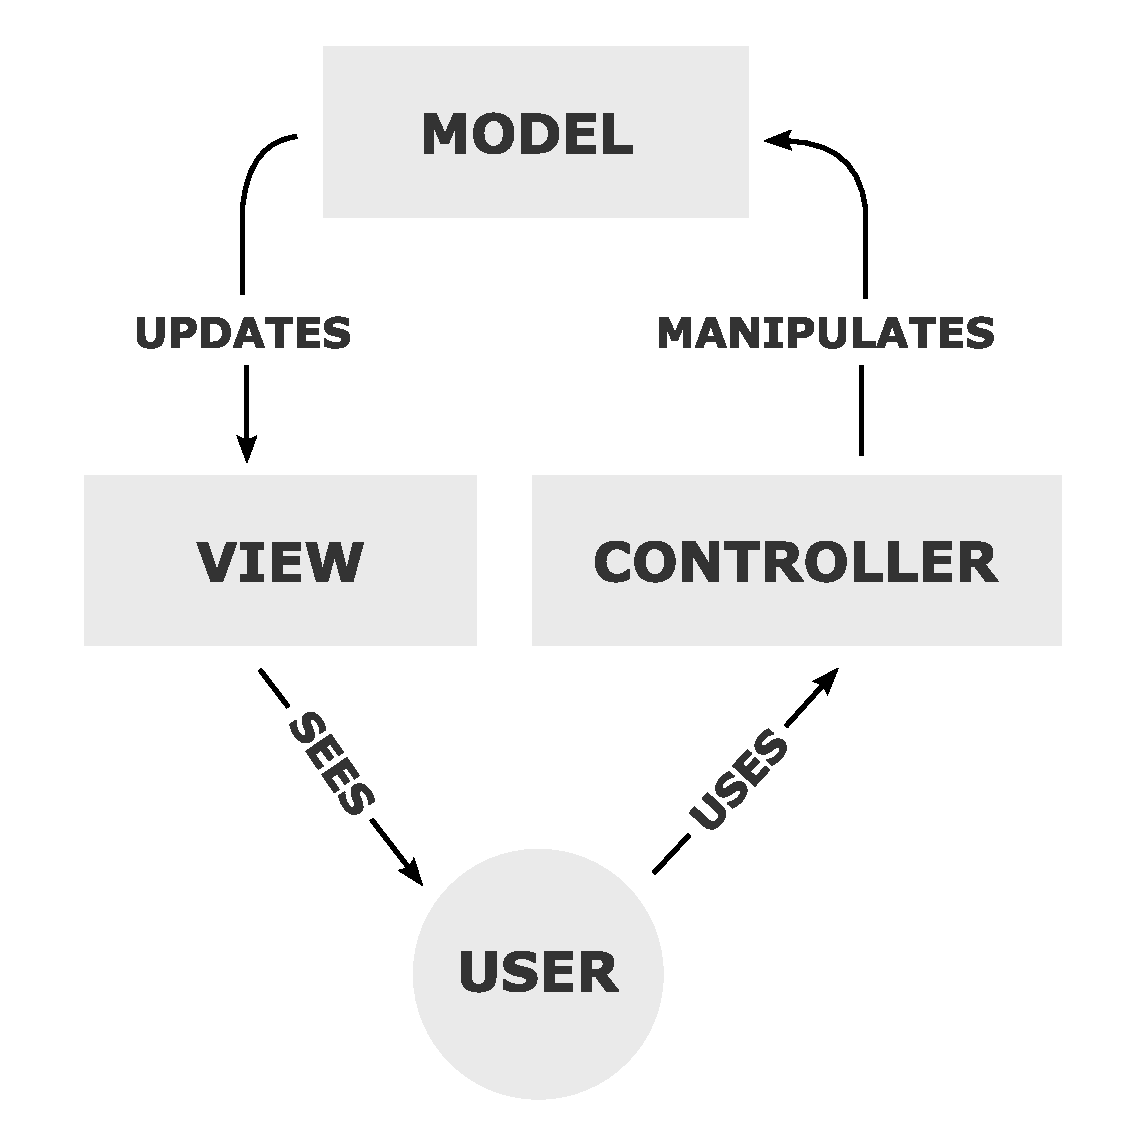
\includegraphics[width=0.75\textwidth]{mvc.pdf}
  \caption{Grundidéen omkring MVC. Fra \url{http://commons.wikimedia.org/wiki/File:MVC-Process.svg} } \label{fig:mvc}
\end{figure}



\section{Database} 
\label{sec:database}

En database er en organisering af en mængde data, ved brug af tabeller. En database bruges til at håndtere opgaver såsom, at gemme, hente eller søge i ofte store mængder lagrede data. En normal fil kan ikke skrives til, fra flere processer på samme tid, hvor en database derimod kan håndtere anmodninger fra flere aktører synkront. Et krav til løsningen er muligheden for at flere bruger kan anvende systemet på samme tid. Derfor skal flere instanser af programmet, have mulighed for at tilgå den samme data både synkront og asynkront. Dette er en væsentlig funktionalitet som anvendelse af en database tilføjer til programmet \cite{DatabaseMicosoftOffice}. 

\subsection{Databasetransaktion}
\label{sub:databasetransaktion}

Hver gang man udfører en eller flere operation på databasen, benyttes en databasetransaktion, for at sikre, at alle operationerne udføres. En databasetransaktion er en gruppering af operationer, som databasen betragter som en samlet enhed. Denne gruppering udgør en mængde operationer, hvor ingen af operationerne skal udføres uden de andre. Såfremt en operation fejler fortrydes alle andre operationer i grupperingen. Dette gøres for at opretholde en synkronisering mellem sammenhængende data \cite{databasetransaktion}.

\subsection{ACID}
\label{sub:acid}

ACID er et akronym for et sæt af forudsætninger, som sikrer at en database fungerer, som beskrevet tidligere, ved samtlige databasetransaktioner. Sættet består af følgende fire forudsætninger: 

\begin{itemize}
	\item \textbf{Atomar - (Atomicity)} \\
		Hvis én operation slår fejl, skal alle operationer i transaktionen tilbageføres, så database har samme tilstand som før transaktionens start. 

	\item \textbf{Konsistens - (Consistency)} \\
		Alt data skal valideres før det skrives til databasen. Dette skal sikre at alt data fra transaktion, er valideret før nogen anden del af data gemmes. Derved sikres at databasen, altid forbliver i en valideret tilstand.

	\item \textbf{Isolering - (Isolation)} \\
		Transaktionerne skal udføres sekventielt og isoleret fra hinanden. En transaktion må ikke kunne se ændringer fra en anden ufuldendt transaktion. Ved at udføre alle transaktion sekventielt sikres det at en transaktion ikke benytter sig af ugyldigt data fra en anden transaktion.

	\item \textbf{Varighed - (Durability)} \\
		Når en transaktion er udført, skal den gemmes på en permanent lagerplads. Selv hvis strømmen går skal alle effekterne af transaktionen være udført.
\end{itemize}

% subsection acid (end)

\subsection{Database}
\label{sub:database}



\section{Windows Presentation Foundation}
\label{sec:wpf}

Windows Presentation Foundation (WPF) er et framework til at udvikle brugergrænseflader til Windows .NET platformen. Kernen i WPF er en vektor-baseret layout-motor. Udover kernen har WPF yderligere funktioner, der inkluderer databinding, templates, animation, medie-services med mere. I dette projekt benyttes WPF's databinding og template funktioner. Disse vil blive beskrevet i dette afsnit.

I WPF består en brugergrænseflade af nogle visuelle elementer, som beskrives ved hjælp af opmærkningssproget XAML. Sammen med XAML-filen, hører en \enquote{Code-behind} fil. I denne C\# klasse kan eventuel logik tilhørende XAML filen programmeres. På den måde adskille udseende og adfærd \cite{microsoft_wpf}.

\subsection{Databinding}

Databinding er en process, der forbinder en brugergrænseflade med programlogik. Fordelen ved at bruge databinding er, at brugergrænsefladen kan kodes separeres fra programlogikken. På den måde opnås en lav kobling mellem komponenterne.

Med databinding kan modeller, beskrevet som C\# klasser, direkte inkorporeres i brugergrænsefladen. Ved brug af events som INotifyPropertyChanged, der kaldes når en egenskab ændres, sørger WPF selv for at opdatere informationen, der vises i brugergrænsefladen, så den svarer til modellen. Hvis der bruges en tovejs binding, vil data i modellen blive opdateret, efter hvad brugen indtaster i grænsefladen.

For at databinde brugergrænsefladen til en model, sættes \enquote{DataContext} egenskaben til at referere, til klassen der skal benyttes som model. I XAML-filen kan modellens egenskaber og felter, nu benyttes til, at vise eller modtage informationer.

\subsection{Templates}

For at begrænse duplikering af kode, kan ofte brugte WPF elementer flyttes ud i en ekstern fil. På den måde kan WPF elementer, benytte samme funktionaliteter eller visuelle elementer, uden at allerede skrevet kode skal gentages. En template konstrueres, ved nedarvning fra WPF klassen \enquote{UserControl}. I den tilhørende XAML fil, skrives nu de ønskede visuelle elementer der skal kunne genbruges.

